% PART 2 -- 15 slides / 15 minutes. Include inside a Beamer document.
% Official figures retain source content; crops/conversions are documented.
\begingroup
% All diagram styles are local to the group opened by part2_topology.tex.
% TikZ styles for the remaining author-created explanatory diagrams.
% Official source images are included directly by part2_topology.tex.
\tikzset{
 pTwo/base/.style={font=\small,align=center,inner sep=4pt},
 pTwo/box/.style={pTwo/base,draw=BKTemplate,fill=BKTemplate!7,line width=.7pt},
 pTwo/gpu/.style={pTwo/box,minimum width=1.05cm,minimum height=.58cm},
 pTwo/domain/.style={pTwo/base,draw=BKTemplate!65,fill=white,line width=.6pt},
 pTwo/arrow/.style={-{Stealth[length=2mm]},draw=BKTemplate,line width=.9pt},
 pTwo/link/.style={draw=BKTemplate,line width=1.1pt},
 pTwo/remote/.style={draw=orange!80!black,line width=1.1pt,dashed},
 pTwo/selected/.style={pTwo/gpu,fill=BKTemplate,text=white},
 pTwo/empty/.style={pTwo/gpu,draw=gray!65,fill=gray!8,text=gray!75!black},
 pTwo/label/.style={font=\small,align=center,text=BKTemplate},
 pTwo/note/.style={font=\small,align=center}
}
% Keep source metadata in TeX without displaying it on slides.
\newcommand{\PtwoSource}[1]{}
\newcommand{\PtwoPoint}[1]{%
 \begin{block}{}\centering #1\end{block}}

\section[Distributed Training \& TAS]{Distributed Training \& Topology-Aware Scheduling}
\subsection{A -- Distributed Training Communication}

% 01 -- 1:10
\begin{frame}{Data Parallelism và Model Parallelism}
 \small
 \textbf{Distributed Training: nhiều GPU workers cùng thực hiện một training job.}
 \par\vspace{.12cm}
 \begin{center}
  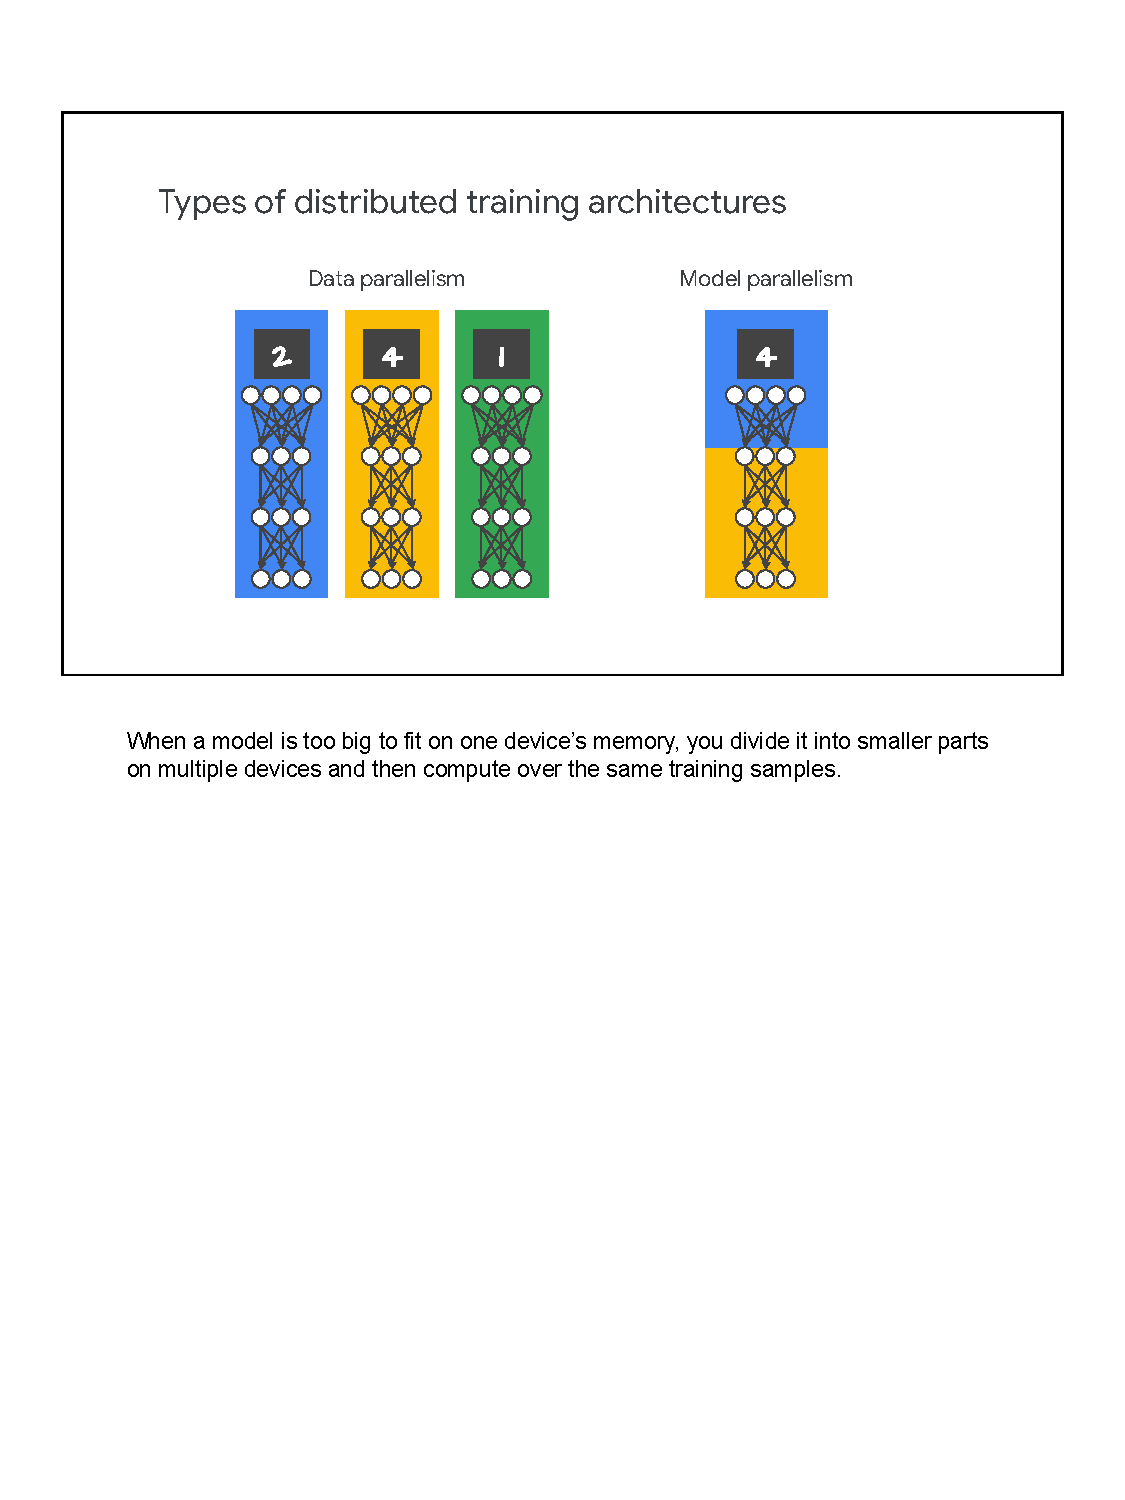
\includegraphics[height=3.8cm,width=.8\linewidth,keepaspectratio,
   trim=100bp 425bp 115bp 120bp,clip]{figures/part2/official/google_parallelism_page_57.pdf}
 \end{center}
 \vspace{-.15cm}
 \begin{columns}[T,onlytextwidth]
  \begin{column}{.48\textwidth}
   \textbf{Data Parallelism}: cùng model, khác dữ liệu.
  \end{column}
  \begin{column}{.48\textwidth}
   \textbf{Model Parallelism}: chia model giữa GPUs.
  \end{column}
 \end{columns}
 \par\vspace{.16cm}Nhiều GPU cung cấp thêm compute; chia model giúp đáp ứng giới hạn bộ nhớ.
 \PtwoSource{Hình: \href{https://storage.googleapis.com/cloud-training/T-PSML-O/on-demand/T-PSML-O_M3_Designing_High-performance_ML_systems.pdf\#page=57}{[R13] Google Cloud Training, Module 03, tr. 57} (trích vùng biểu đồ).}
\end{frame}

% 02 -- 0:55
\begin{frame}{GPU Workers trong một Training Step}
 \small
 \begin{columns}[c,onlytextwidth]
  \begin{column}{.46\textwidth}
   \textbf{Ví dụ synchronous Data Parallelism}
   \begin{enumerate}
    \setlength{\itemsep}{.22cm}
    \item Nhận phần mini-batch riêng.
    \item \textbf{Forward}: tính outputs và loss.
    \item \textbf{Backward}: tính gradients.
    \item Đồng bộ gradients, rồi update model.
   \end{enumerate}
  \end{column}
  \begin{column}{.5\textwidth}
   \colorbox{white}{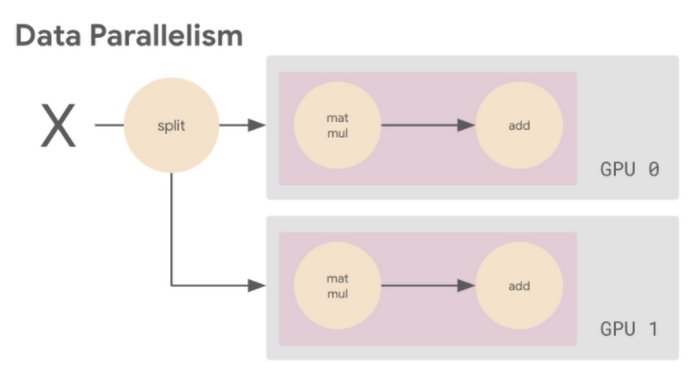
\includegraphics[width=.96\linewidth]{figures/part2/official/google_cloud_data_parallelism.png}}
   \par\vspace{.12cm}Hình: input $X$ chia cho GPU 0 và GPU 1.
  \end{column}
 \end{columns}
 \PtwoPoint{Worker thực hiện compute cục bộ và phối hợp với các workers khác.}
 \PtwoSource{Hình: \href{https://cloud.google.com/blog/topics/developers-practitioners/optimize-training-performance-reduction-server-vertex-ai}{[R14] Google Cloud Blog}; cơ chế Backward/sync: [R1] PyTorch DDP.}
\end{frame}

% 03 -- 1:05
\begin{frame}{Gradient Synchronization với AllReduce}
 \small
 \textbf{Mỗi worker có gradient cục bộ; mọi worker cần cùng kết quả tổng hợp.}
 \begin{center}
  \colorbox{white}{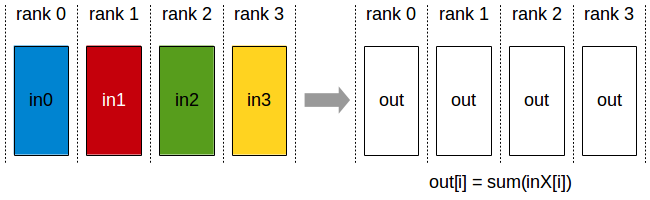
\includegraphics[width=10.8cm]{figures/part2/official/nvidia_nccl_allreduce.png}}
 \end{center}
 \begin{columns}[T,onlytextwidth]
  \begin{column}{.48\textwidth}
   \textbf{Trong hình NVIDIA: Sum AllReduce}\\
   Mỗi rank nhận cùng $g_{\mathrm{sum}}=\sum_{i=0}^{3} g_i$.
  \end{column}
  \begin{column}{.48\textwidth}
   \textbf{Ví dụ gradient trung bình}\\
   Với local batch bằng nhau: $\bar g=g_{\mathrm{sum}}/4$.
  \end{column}
 \end{columns}
 \PtwoPoint{NCCL cung cấp collective communication; AllReduce không cần parameter server.}
 \PtwoSource{Hình: \href{https://docs.nvidia.com/deeplearning/nccl/user-guide/docs/usage/collectives.html\#allreduce}{[R2] NVIDIA NCCL User Guide: AllReduce}.}
\end{frame}

% 04 -- 0:50
\begin{frame}{ReduceScatter và AllGather}
 \small
 \textbf{Có thể phân rã AllReduce thành hai collective operations:}
 \par\vspace{.3cm}
 \begin{columns}[T,onlytextwidth]
  \begin{column}{.48\textwidth}
   \centering\textbf{1. ReduceScatter}
   \par\vspace{.18cm}
   \colorbox{white}{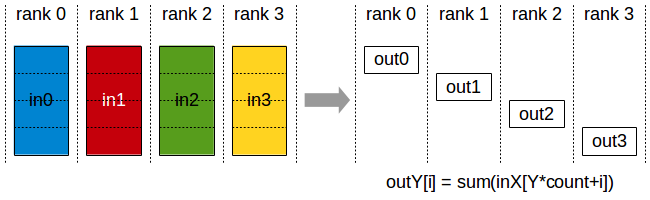
\includegraphics[width=.96\linewidth]{figures/part2/official/nvidia_nccl_reducescatter.png}}
   \par\vspace{.2cm}Mỗi rank giữ một phần của kết quả reduction.
  \end{column}
  \begin{column}{.48\textwidth}
   \centering\textbf{2. AllGather}
   \par\vspace{.18cm}
   \colorbox{white}{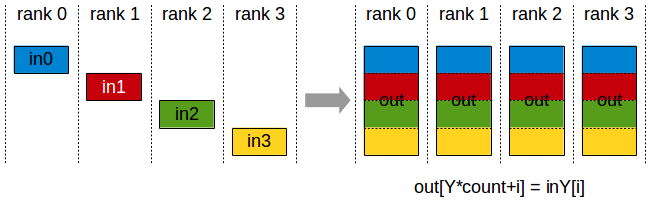
\includegraphics[width=.96\linewidth]{figures/part2/official/nvidia_nccl_allgather.png}}
   \par\vspace{.2cm}Các phần được tập hợp lại trên mọi rank.
  \end{column}
 \end{columns}
 \PtwoPoint{Các hình mô tả semantics; NCCL chọn thuật toán theo topology và cấu hình.}
 \PtwoSource{Hình: \href{https://docs.nvidia.com/deeplearning/nccl/user-guide/docs/usage/collectives.html}{[R2] NVIDIA NCCL User Guide: ReduceScatter / AllGather}.}
\end{frame}

% 05 -- 1:00
\begin{frame}{Vì sao Communication làm tăng Step Time?}
 \small
 \begin{block}{Một training step có cả compute và communication}
  Gradient sync có thể \textbf{overlap} với Backward. Phần chưa được che vẫn nằm trên đường găng.
 \end{block}
 \par\vspace{.2cm}
 \begin{itemize}
  \setlength{\itemsep}{.28cm}
  \item \textbf{Truyền chậm}: kết quả collective hoàn thành muộn hơn.
  \item \textbf{Worker chậm}: các workers khác có thể phải chờ đồng bộ.
  \item \textbf{Thêm GPU}: tăng compute capacity, đồng thời phát sinh trao đổi.
 \end{itemize}
 \PtwoPoint{Communication là nút thắt $\Rightarrow$ thêm GPU chưa chắc giảm training time.}
 \PtwoSource{\href{https://docs.pytorch.org/tutorials/intermediate/ddp_tutorial.html}{[R1] PyTorch DDP}; \href{https://docs.pytorch.org/docs/2.15/notes/ddp.html}{[R12] DDP design note}.}
\end{frame}

\subsection{B -- GPU Cluster Topology}

% 06 -- 0:55
\begin{frame}{GPU Node, Rack, Block và Cluster}
 \small
 \centering% Generic hierarchy. No assertion that these are real GKE labels or one SKU.
\begin{tikzpicture}[x=1cm,y=1cm]
 \node[pTwo/label,font=\small\bfseries] at (7,4.15) {Cluster: nhiều topology domains};
 \draw[pTwo/domain] (.15,.35) rectangle (13.85,3.72);
 \node[pTwo/label,fill=white] at (7,3.72) {Block A};
 \foreach \base/\rack in {.45/A,7.45/B}{
  \draw[pTwo/domain] (\base,.65) rectangle ++(5.9,2.7);
  \node[pTwo/label] at (\base+2.95,3.08) {Rack \rack};
  \foreach \offset/\idx in {.25/1,3.15/2}{
   \draw[pTwo/box] (\base+\offset,1.1) rectangle ++(2.5,1.55);
   \node[pTwo/note] at (\base+\offset+1.25,2.35) {Node \rack\idx};
   \node[pTwo/gpu,minimum width=.8cm] (g\rack\idx a) at (\base+\offset+.65,1.65) {GPU};
   \node[pTwo/gpu,minimum width=.8cm] (g\rack\idx b) at (\base+\offset+1.85,1.65) {GPU};
   \draw[pTwo/link] (g\rack\idx a) -- (g\rack\idx b);
   \draw[pTwo/link] (\base+\offset+1.25,1.1) -- (\base+\offset+1.25,.9);
  }
  \draw[pTwo/link] (\base+1.5,.9) -- (\base+4.4,.9);
 }
 \draw[pTwo/remote] (4.85,.9) -- (8.95,.9);
 \node[pTwo/note] at (3.4,-.02) {Intra-node: PCIe / NVLink; NVSwitch tùy hệ thống};
 \node[pTwo/note] at (10.5,-.02) {Inter-node: NIC $\leftrightarrow$ mạng cluster};
\end{tikzpicture}

 \par\vspace{.18cm}
 \begin{columns}[T,onlytextwidth]
  \begin{column}{.48\textwidth}
   \textbf{Node}: máy/VM chứa GPUs.\\
   \textbf{Rack}: nhóm các máy trong một tủ rack.
  \end{column}
  \begin{column}{.48\textwidth}
   \textbf{Block}: nhóm racks theo mô hình cluster.\\
   \textbf{Cluster}: tập hợp các nodes và kết nối mạng.
  \end{column}
 \end{columns}
 \PtwoSource{Sơ đồ tác giả, mô hình tổng quát theo \href{https://github.com/kubernetes-sigs/kueue/blob/v0.14.0/site/content/en/docs/concepts/topology_aware_scheduling.md}{[R6] Kueue TAS}; không đại diện một GPU SKU cụ thể.}
\end{frame}

% 07 -- 1:10
\begin{frame}{Intra-node: GPU và NVSwitch}
 \small
 \textbf{Ví dụ phần cứng: NVIDIA DGX H100/H200, tám GPUs trong một hệ thống.}
 \begin{center}
  \colorbox{white}{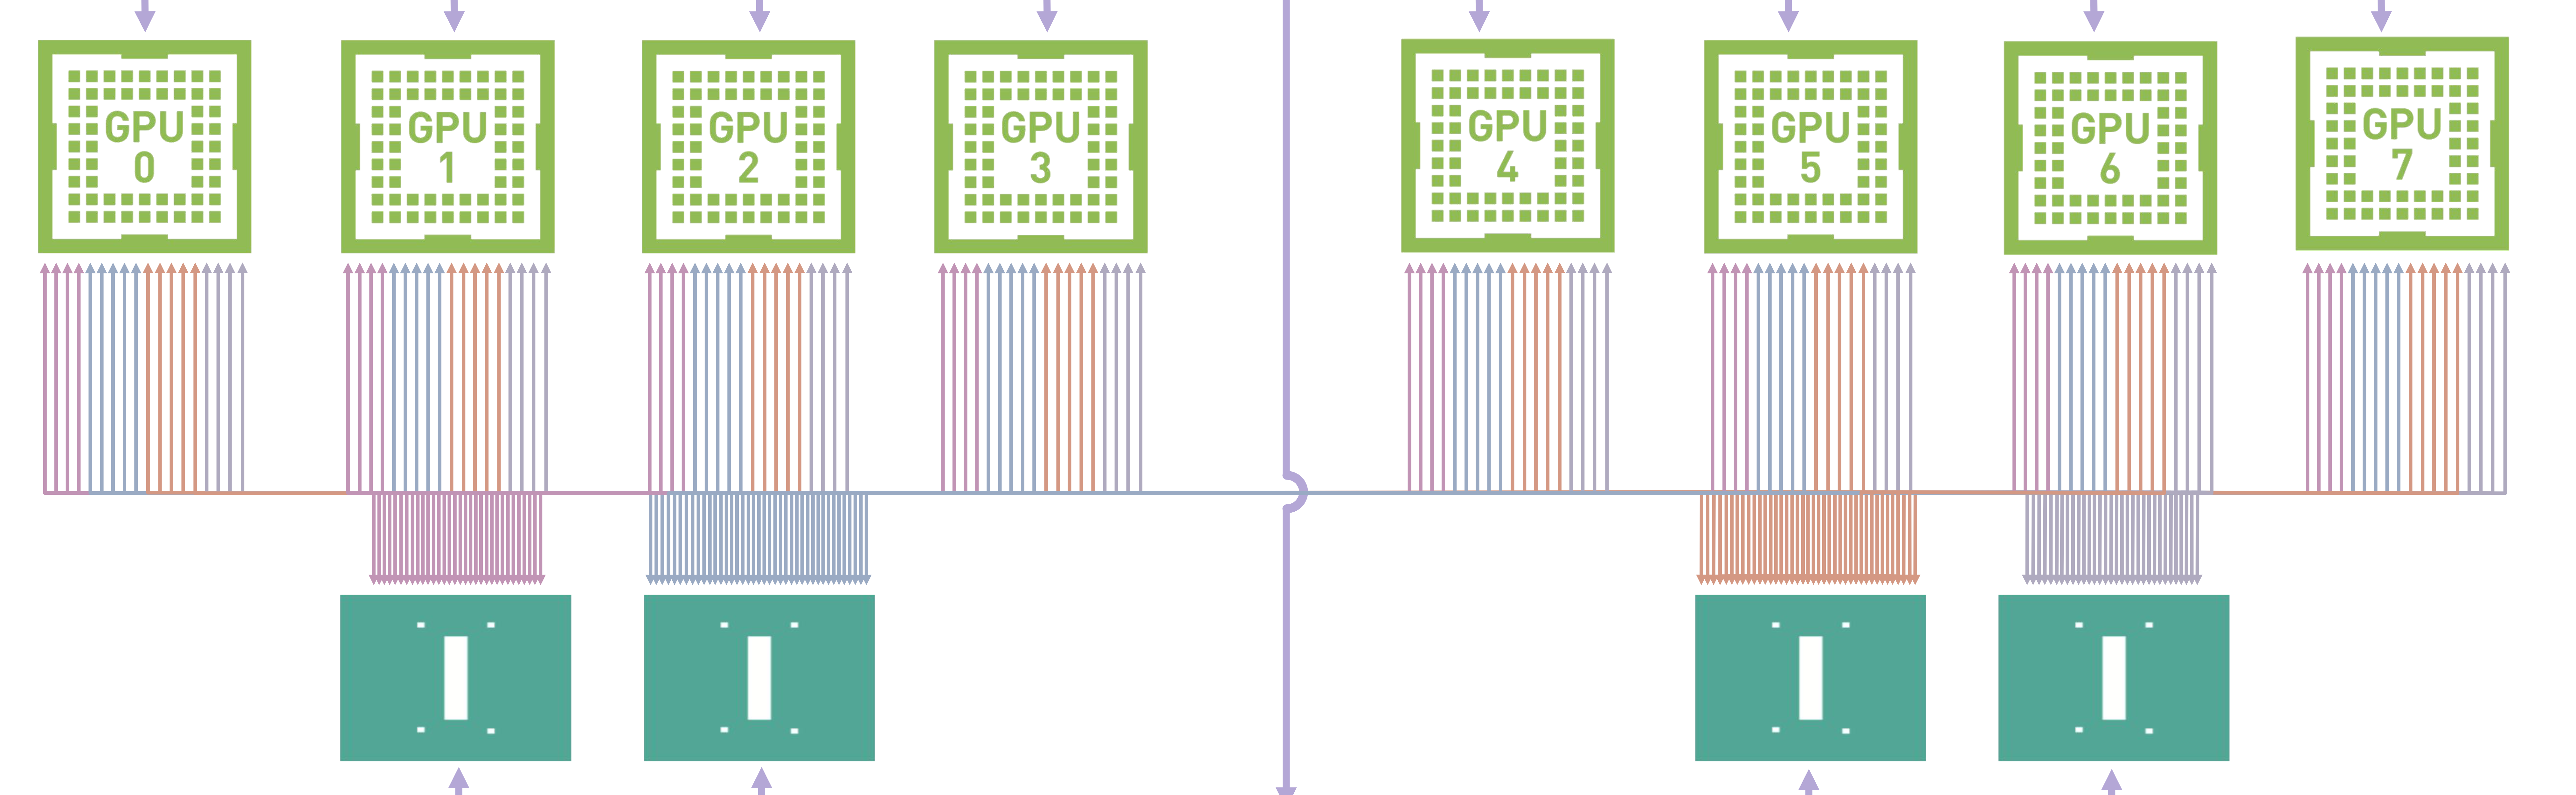
\includegraphics[width=13cm,height=4.05cm,keepaspectratio]{figures/part2/official/nvidia_dgx_gpu_nvswitch_detail.png}}
 \end{center}
 \vspace{-.15cm}
 \begin{columns}[T,onlytextwidth]
  \begin{column}{.48\textwidth}
   \textbf{GPU (xanh lá) $\leftrightarrow$ NVSwitch (xanh ngọc)}\\
   NVSwitch kết nối GPUs trong NVLink fabric.
  \end{column}
  \begin{column}{.48\textwidth}
   PCIe kết nối các thành phần I/O của hệ thống.\\
   Interconnect thực tế phụ thuộc phần cứng.
  \end{column}
 \end{columns}
 \PtwoSource{Hình: \href{https://docs.nvidia.com/dgx/dgxh100-user-guide/introduction-to-dgxh100.html\#dgx-h100-200-system-topology}{[R15] NVIDIA DGX H100/H200 User Guide} (trích vùng GPU/NVSwitch; không phải sơ đồ GKE).}
\end{frame}

% 08 -- 1:05
\begin{frame}{Inter-node Communication trên Google Cloud}
 \small
 \textbf{Ví dụ chính thức: A3 Ultra / A4 với các network planes riêng.}
 \begin{center}
  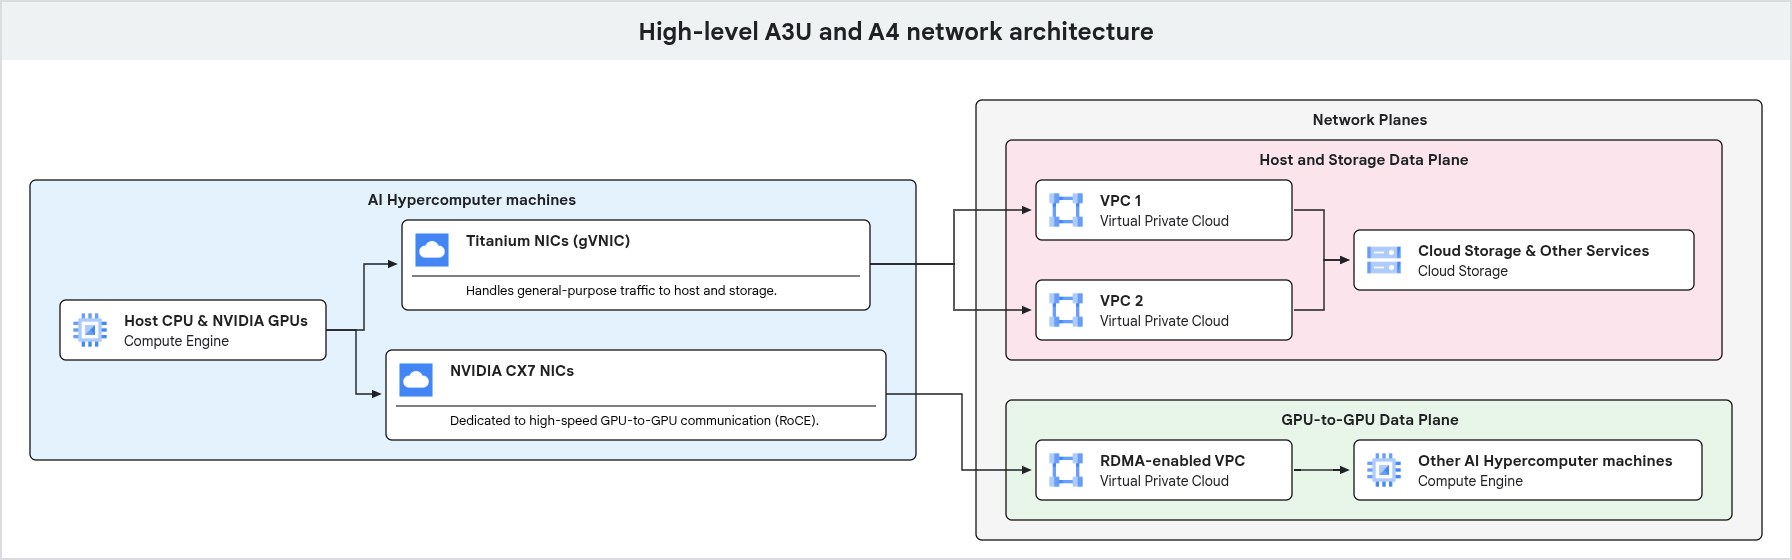
\includegraphics[width=14.3cm,height=4.5cm,keepaspectratio]{figures/part2/official/google_gpu_network_architecture.png}
 \end{center}
 \vspace{-.15cm}
 \begin{columns}[T,onlytextwidth]
  \begin{column}{.48\textwidth}
   \textbf{Titanium NICs}: host / storage traffic.
  \end{column}
  \begin{column}{.48\textwidth}
   \textbf{CX7 NICs + RDMA VPC}: GPU-to-GPU traffic.
  \end{column}
 \end{columns}
 \par\vspace{.15cm}Ethernet/RoCE và InfiniBand là các lựa chọn trong GPU clusters; hình này dùng RoCE.
 \PtwoSource{Hình: \href{https://docs.cloud.google.com/ai-hypercomputer/docs/networking-overview}{[R16] Google Cloud: GPU networking overview}; cấu hình tùy machine type.}
\end{frame}

% 09 -- 0:50
\begin{frame}{Bandwidth, Latency và Communication Overhead}
 \small
 \begin{tabular}{@{}p{3cm}p{10.9cm}@{}}
  \toprule
  \textbf{Đại lượng} & \textbf{Ảnh hưởng đến giao tiếp}\\\midrule
  Bandwidth & Khả năng truyền dữ liệu mỗi giây; quan trọng với gradient tensors lớn.\\[.18cm]
  Latency & Chi phí khởi đầu/độ trễ của một trao đổi; đáng kể khi lặp nhiều trao đổi ngắn.\\[.18cm]
  Contention & Các luồng traffic cạnh tranh trên liên kết hoặc tài nguyên dùng chung.\\\bottomrule
 \end{tabular}
 \par\vspace{.35cm}
 \textbf{Intra-node} và \textbf{inter-node} đi qua các đường phần cứng khác nhau.\\[.12cm]
 Cùng số GPU nhưng khác placement có thể tạo communication overhead khác nhau.
 \PtwoPoint{Cần xem interconnect và workload cụ thể; không có một hệ số nhanh/chậm chung.}
 \PtwoSource{\href{https://docs.nvidia.com/deeplearning/nccl/user-guide/docs/overview.html}{[R5] NVIDIA NCCL Overview}; [R4] Compute Engine GPU machines; [R16] Google Cloud networking.}
\end{frame}

\subsection{C -- Topology-Aware Scheduling}

% 10 -- 1:00
\begin{frame}{Topology-Aware Scheduling: Availability và Locality}
 \small
 \textbf{Availability}: còn bao nhiêu tài nguyên?\quad\textbf{Locality}: chúng nằm ở đâu?
 \par\vspace{.3cm}
 \begin{columns}[c,onlytextwidth]
  \begin{column}{.48\textwidth}
   \centering% Availability snapshot for eight Pods, each requesting one GPU.
\begin{tikzpicture}[x=1cm,y=1cm]
 \node[pTwo/box,minimum width=4.5cm] (b) at (3.1,3.55) {Block A: 12 GPU trống};
 \node[pTwo/box,minimum width=2.5cm] (r1) at (1.5,2.5) {Rack A: 6 GPU};
 \node[pTwo/box,minimum width=2.5cm] (r2) at (4.8,2.5) {Rack B: 6 GPU};
 \draw[pTwo/arrow] (b) -- (r1);
 \draw[pTwo/arrow] (b) -- (r2);
 \foreach \x/\n in {.65/A1,2.35/A2,3.95/B1,5.65/B2}{
  \node[pTwo/box,minimum width=1.35cm,minimum height=.85cm,inner sep=2pt] (n\n) at (\x,1.25) {Node \n\\3 GPU};
 }
 \draw[pTwo/arrow] (r1) -- (nA1);
 \draw[pTwo/arrow] (r1) -- (nA2);
 \draw[pTwo/arrow] (r2) -- (nB1);
 \draw[pTwo/arrow] (r2) -- (nB2);
 \node[pTwo/note,text width=6.3cm] at (3.1,.25) {Job cần 8 GPU: đủ tổng capacity,\\nhưng không rack nào chứa đủ 8 workers.};
\end{tikzpicture}

  \end{column}
  \begin{column}{.48\textwidth}
   \textbf{Topology-Aware Scheduling}\\
   Xét capacity cùng cấu trúc topology khi chọn domain cho workers.
   \par\vspace{.3cm}
   \textbf{Ví dụ: job cần 8 GPU}\\
   Tổng còn 12 GPU, nhưng mỗi rack chỉ còn 6.
   \par\vspace{.25cm}
   Đủ tổng GPU chưa bảo đảm đủ chỗ trong domain mong muốn.
  \end{column}
 \end{columns}
 \PtwoSource{Sơ đồ minh họa của tác giả theo \href{https://github.com/kubernetes-sigs/kueue/blob/v0.14.0/site/content/en/docs/concepts/topology_aware_scheduling.md}{[R6] Kueue TAS v0.14.0}; quota, CPU và RAM giả định đủ.}
\end{frame}

% 11 -- 0:55
\begin{frame}{Required và Preferred Topology}
 \small
 \begin{columns}[T,onlytextwidth]
  \begin{column}{.48\textwidth}
   \begin{block}{Required: phải cùng một rack}
    Mỗi rack còn 6 GPU, job cần 8.\\[.18cm]
    Không domain nào đủ $\Rightarrow$ chờ admission.
   \end{block}
  \end{column}
  \begin{column}{.48\textwidth}
   \begin{block}{Preferred: ưu tiên cùng một rack}
    Không vừa rack $\Rightarrow$ xét cấp rộng hơn.\\[.18cm]
    Block còn 12 GPU: có thể chứa 8 workers.
   \end{block}
  \end{column}
 \end{columns}
 \par\vspace{.3cm}
 \textbf{Lợi ích}: chọn locality phù hợp với nhu cầu communication.\\[.18cm]
 \textbf{Giới hạn}: locality chặt hơn có thể tăng thời gian chờ; không bảo đảm speedup.
 \PtwoPoint{Preferred là fallback theo cấp topology; không phải timeout để bỏ Required.}
 \PtwoSource{\href{https://github.com/kubernetes-sigs/kueue/blob/v0.14.0/site/content/en/docs/concepts/topology_aware_scheduling.md}{[R6] Kueue v0.14.0: User-facing APIs}; [R8] PodSetTopologyRequest.}
\end{frame}

% 12 -- 1:05
\begin{frame}{Kueue: luồng Admission tổng quan}
 \small
 \textbf{Admin chuẩn bị flavors/queues; user gửi job qua Kubernetes API.}
 \begin{center}
  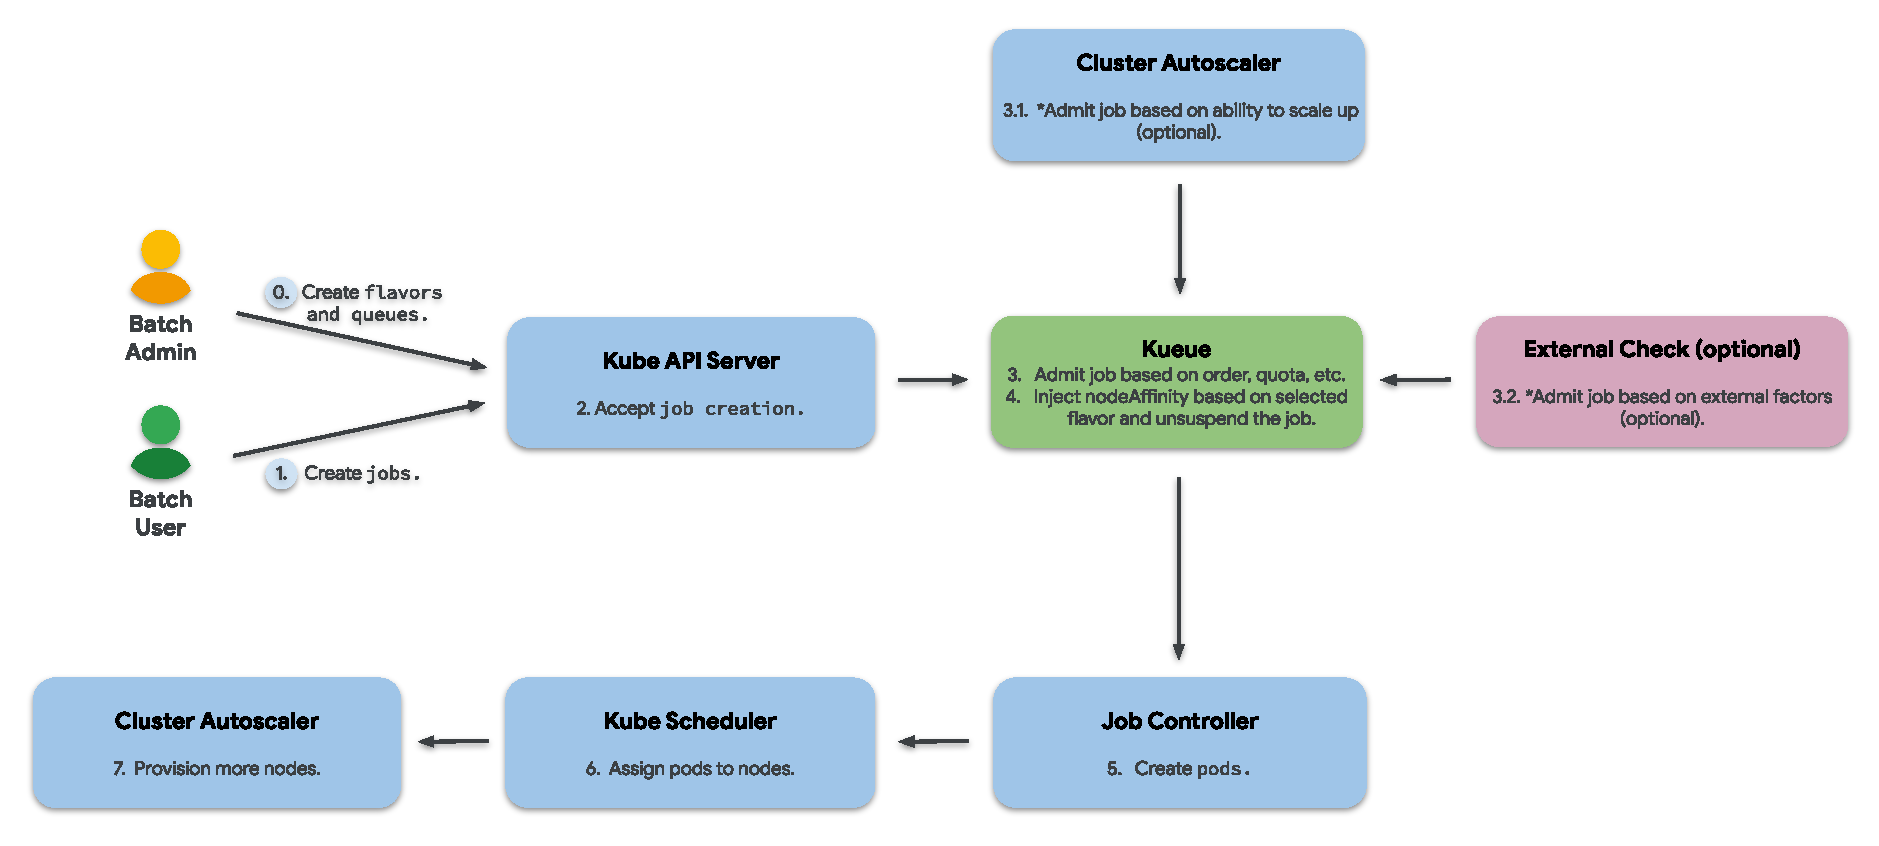
\includegraphics[width=14.3cm,trim=0bp 132bp 0bp 85bp,clip]{figures/part2/official/kueue_theory_of_operation.pdf}
 \end{center}
 \vspace{-.15cm}
 \begin{itemize}
  \setlength{\itemsep}{.15cm}
  \item \textbf{Kueue}: xét admission theo quota và chính sách; áp ràng buộc tài nguyên.
  \item \textbf{Sau admission}: Job Controller tạo Pods; kube-scheduler thực hiện binding.
  \item Autoscaling / external checks là tùy chọn; \textbf{TAS ở slide tiếp theo}.
 \end{itemize}
 \PtwoSource{Hình: \href{https://kueue.sigs.k8s.io/docs/overview/\#high-level-kueue-operation}{[R17] Kueue Documentation: High-level operation} (trích vùng admission từ PDF vector).}
\end{frame}

% 13 -- 1:15
\begin{frame}{Kueue TAS: Admission đến Pod Placement}
 \small
 \textbf{Kueue v0.14.0}: TAS Beta, bật mặc định; API \texttt{kueue.x-k8s.io/v1beta1}.
 \begin{center}% Kueue v0.14.0, existing capacity, no Provisioning AdmissionCheck in this flow.
\begin{tikzpicture}[x=1cm,y=1cm]
 \node[pTwo/box,text width=5.3cm,minimum height=.95cm] (admin) at (3.05,4.1) {Topology $\leftarrow$ ResourceFlavor\\Admin: queues + quota};
 \node[pTwo/box,text width=5.3cm,minimum height=.95cm] (user) at (10.75,4.1) {User: Job + annotation\\PodTemplate $\rightarrow$ PodSet};
 \node[pTwo/box,text width=11.7cm,minimum height=.9cm] (admit) at (6.9,2.62) {Kueue: kiểm tra quota + topology capacity\\Admission + topology assignment cho PodSet};
 \draw[pTwo/arrow] (admin.south) -- (3.05,3.2);
 \draw[pTwo/arrow] (user.south) -- (10.75,3.2);
 \node[pTwo/box,text width=11.7cm,minimum height=.85cm] (pod) at (6.9,1.22) {Controllers: tạo Pods; áp node selectors theo assignment\\Kueue TAS controller gỡ topology scheduling gate};
 \draw[pTwo/arrow] (admit) -- (pod);
 \node[pTwo/box,text width=11.7cm,minimum height=.6cm] (sched) at (6.9,-.02) {kube-scheduler: Filter / Score $\rightarrow$ Bind Pod vào Node phù hợp};
 \draw[pTwo/arrow] (pod) -- (sched);
\end{tikzpicture}
\end{center}
 \vspace{-.15cm}
 \textbf{PodTemplate annotation:}\quad\texttt{kueue.x-k8s.io/podset-required-topology}
 \par\vspace{.1cm}Kueue chọn topology assignment; \textbf{kube-scheduler thực hiện Pod binding}.
 \PtwoSource{Sơ đồ tác giả; [R7--R10] Kueue v0.14.0; [R11] Kubernetes Scheduler.}
\end{frame}

% 14 -- 1:05
\begin{frame}{Case Study: 8-GPU Worker Placement}
 \small
 \textbf{8 workers $\times$ 1 GPU}; 2 racks $\times$ 2 nodes/rack $\times$ 4 GPU trống/node.
 \par\vspace{.12cm}{\centering% Same capacity snapshot in both panels: four nodes, four free GPUs each.
% Filled positions = job's workers, outlined positions = unused GPUs.
\begin{tikzpicture}[x=1cm,y=1cm]
 \foreach \base/\title in {0/{Topology-Aware: 1 rack},7.05/{Topology-Unaware: 2 racks}}{
  \node[pTwo/label,font=\small\bfseries] at (\base+3.25,3.35) {\title};
  \foreach \offset/\rack in {.1/A,3.55/B}{
   \draw[pTwo/domain] (\base+\offset,.4) rectangle ++(2.85,2.5);
   \node[pTwo/label] at (\base+\offset+1.425,2.62) {Rack \rack};
   \foreach \row/\idx in {1.95/1,.95/2}{
    \node[font=\small,anchor=west] at (\base+\offset+.1,\row+.28) {Node \rack\idx};
    \foreach \col in {0,1,2,3}{
     \node[pTwo/empty,minimum width=.48cm,minimum height=.43cm,inner sep=0pt] at (\base+\offset+.55+\col*.58,\row-.15) {};
    }
   }
  }
 }
 \foreach \row in {1.95,.95}{
  \foreach \col in {0,1,2,3}{
   \node[pTwo/selected,minimum width=.48cm,minimum height=.43cm,inner sep=0pt] at (.65+\col*.58,\row-.15) {W};
  }
  \foreach \offset in {7.15,10.6}{
   \foreach \col in {0,1}{
    \node[pTwo/selected,minimum width=.48cm,minimum height=.43cm,inner sep=0pt] at (\offset+.55+\col*.58,\row-.15) {W};
   }
  }
 }
 \draw[pTwo/remote] (9.95,1.65) -- (10.6,1.65);
 \node[pTwo/note] at (3.25,-.02) {4 + 4 workers trên 2 nodes};
 \node[pTwo/note] at (10.3,-.02) {2 + 2 + 2 + 2 workers trên 4 nodes};
\end{tikzpicture}
\par}\vspace{.08cm}
 \textcolor{BKTemplate}{\rule{.22cm}{.22cm}}\; Worker của job\qquad
 \fbox{\rule{0pt}{.14cm}\hspace{.14cm}}\; GPU chưa dùng
 \par\vspace{.02cm}
 Cùng rack có thể giảm overhead \textbf{nếu liên kết xuyên rack là nút thắt}.
 \PtwoPoint{Kịch bản tự xây dựng, không phải benchmark; không suy ra mức speedup.}
 \PtwoSource{Sơ đồ tác giả theo [R6] Kueue TAS v0.14.0.}
\end{frame}

% 15 -- 0:40
\begin{frame}{Key Takeaways}
 \small
 \begin{itemize}
  \setlength{\itemsep}{.18cm}
  \item Distributed Training cần \textbf{compute và communication}.
  \item Topology-Aware Scheduling kết hợp \textbf{capacity với locality}.
  \item Kueue hỗ trợ topology-aware admission; kube-scheduler bind Pods.
 \end{itemize}
 \begin{block}{Thông điệp kết thúc}
  \textbf{Có đủ GPU chưa chắc đã đủ; vị trí của các GPU cũng quyết định hiệu quả huấn luyện phân tán.}
 \end{block}
 \par\vspace{.18cm}
 Sau khi xác định khi nào workload được chạy và các GPU workers nên được đặt ở đâu,
 vấn đề tiếp theo là làm thế nào để sử dụng và chia sẻ GPU hiệu quả hơn?
 \PtwoSource{[R1] PyTorch DDP; [R6] Kueue TAS; [R11] Kubernetes Scheduler.}
\end{frame}
\endgroup
